\section{Bayesian inference of parameters}

\subsection{Bayesian inference - an introduction}
(is it necessary?) Introduction of Bayesian inference, concluding with
\begin{equation}\label{BayesFormula}
	\pi(\theta|d) \propto \mathcal{Q}(\theta) \diffL(d|\theta)
\end{equation}

\subsection{Bayesian inference of the parameters of an ODE}

Let us consider the following initial value problem. Given $u_0$ a vector in $\R^d$ and a parameter set $\theta$ in $\R^p$
\begin{equation}\label{ODEParam}
\begin{aligned}
	\dv{u}{t}\left(t; \theta\right) &= f(u(t;\theta)),\\
	u(0; \theta) &= u_0.
\end{aligned}
\end{equation}
We consider the case in which $\theta$ is not known a priori and the problem of estimating its distribution. We consider the set of data $d_i$ in $\R^d$ with $i = 1, \ldots, D$ which represents the observed state of the system $\eqref{ODEParam}$ at a set of time $t_i, i = 1, \ldots, D$ in which an observational noise $\epl$ is present. We assume that $\epl$ is normally distributed with zero mean and a given variance $\Gamma$, i.e.,
\begin{equation}
	d_i = u(t_i) + \epl_i, \quad \epl_i \sim \mathcal{N}(0, \Gamma).
\end{equation} 
If the solution of \eqref{ODEParam} is computable analytically, then thanks to Bayes theorem we know that once a prior distribution $\mathcal{Q}(\theta)$ is specified, the posterior distribution of $\theta$ is given by Bayes' formula and can be expressed as
\begin{equation}\label{BayesFormulaODE}
	\pi(\theta|d) \propto \mathcal{Q}(\theta) \diffL(d|u(t;\theta)).
\end{equation}
 Under the hypothesis that the observational error is normally distributed, the likelihood function is easy to compute and is given by
 \begin{equation}\label{likelihood}
	 \diffL(d|u(\theta)) \propto \exp\left(\frac{1}{2}\sum_{i=1}^{D}\left(u(t_i;\theta) - d_i\right)^T \Gamma^{-2} \left(u(t_i;\theta) - d_i) \right)\right).
 \end{equation}
 In many cases, the analytical solution of \eqref{ODEParam} is not computable in closed form, therefore one replaces the analytical solution with its numerical approximation, which we denote by $U^{h,0}$. We then replace the analytical solution in the ODE, hoping that it does not spoil the quality of the posterior distribution, i.e.,
 \begin{equation}
	 \mathcal{Q}(\theta) \diffL(d|u(\theta)) \approx \mathcal{Q}(\theta) \diffL(d|U^{h,0}(t;\theta)).
 \end{equation}
 Another approach consists of considering the probabilistic numerical method \eqref{probabilityODE} and a set of realizations of its solution. Let us denote by $U^{h, \sigma}(t, \xi; \theta)$ the numerical solution in this case, where $\sigma$ represents the amount of uncertainty that is introduced with the method (see Assumption \ref{assumption_1} and the following remarks). We then replace the likelihood function in \eqref{BayesFormulaODE} integrating over the random variable $\xi$, thus obtaining the following Bayes' rule
 \begin{equation}
	 	\pi(\theta|d) \propto \mathcal{Q}(\theta) \int{\diffL(d|U^{h,\sigma}(t,\xi;\theta))\dd\xi}.
 \end{equation}
 In \cite{CGS16} the authors claim that using the deterministic numerical solution for the purpose of estimating the parameters leads to unreliable posterior distributions, whilst the approximation of $\pi(\theta|d)$ provided by the probabilistic method takes accordingly into account the error introduced by the numerical solution. \\
 In order to draw from the posterior distribution $\pi(\theta|d)$ one has to perform a Markov Chain Monte Carlo method, which is a class of numerical methods for Bayesian inference, briefly introduced in the following section.
 
\subsection{Markov Chain Monte Carlo methods}

\begin{algorithm}[t]
	\caption{Metropolis-Hastings algorithm.}
	\label{alg:MH}
	\KwData{$\theta_0, N_{it}, d_i, i = 0, \ldots, D$.}
	Compute $\mathcal{Q}(\theta_0)$ and $\diffL(d|\theta_0)$ \;
	\For{$k = 0, \ldots, N_{it}$}{
		Draw $\vartheta$ from $q(\theta_k, \cdot)$ \;
		Compute the probability $\alpha = \min\left\{1, \dfrac{\pi(\vartheta|d)q(\theta_k, \vartheta)}{\pi(\theta_k|d)q(\vartheta, \theta_k)}\right\}$ \; \label{alg:MHProb}
		Draw $u$ from $\mathcal{U}(0, 1)$ \;
		\eIf{$\alpha > u$} {
			Accept $\vartheta$, set $\theta_{k+1} = \vartheta$ \; 
		} {
		Set $\theta_{k+1} = \theta$\;
	}
}
\end{algorithm}

The Markov Chain Monte Carlo (MCMC) methods are a useful tool for performing Bayesian inference. The main idea behind these methods is creating a chain of guesses of a parameter $\theta$ in order to build an approximation of its posterior distribution. \\
One of the most popular MCMC methods is the Metropolis-Hastings (MH) algorithm \cite{KaS05}, presented in pseudo-code in Algorithm \ref{alg:MH}. In this algorithm, the new guess $\vartheta$ of the parameter $\theta$ value is drawn from a proposal function $q(\theta_k, \cdot)$ dependent on the current guess $\theta_k$. Then, the new value $\vartheta$ is included in the chain as $\theta_{k+1}$ with a probability $\alpha$ dependent on the ratio between the posterior distribution evaluated in $\vartheta$ and $\theta$, as in line \ref{alg:MHProb} of Algorithm \ref{alg:MH}. Otherwise, $\theta_{k+1}$ is chosen to be equal to $\theta_k$. \\
Let us remark that if $q(x, y)$ is a symmetric function, then the expression of the probability $\alpha$ at the $k$-th step simplifies to 
\begin{equation}
	\alpha = \min\left\{1, \frac{\pi(\vartheta|d)}{\pi(\theta_k|d)}\right\}.
\end{equation}
This is the case, for example, of a Gaussian proposal distribution, which is a common choice (ADDREF) in case no a priori restriction is imposed on the range of $\theta$. \\
Let us consider the problem of finding the distribution of the parameter $\theta$ defining an ODE. In this case, once the new guess $\vartheta$ is generated from the proposal distribution, it is necessary to solve numerically \eqref{ODEParam} in order to determine the value of the likelihood function. In particular, assuming that the proposal distribution $q$ is symmetric, the value of $\alpha$ at the $k$-th step in this frame reads in case the deterministic solver is adopted
\begin{equation}\label{detAlphaMH}
	\alpha = \min\left\{1, \frac{\mathcal{Q}(\vartheta)\diffL(d|U^{h,0}(t; \vartheta))}{\mathcal{Q}(\theta_k)\diffL(d|U^{h,0}(t; \theta_k))}\right\},
\end{equation} 
while for the probabilistic solver one gets
\begin{equation}\label{probAlphaMH}
	\alpha^{h,\sigma} = \min\left\{1, \frac{\mathcal{Q}(\vartheta)\int{\diffL(d|U^{h,\sigma}(t,\xi; \vartheta))\dd\xi}}{\mathcal{Q}(\theta_k)\int{\diffL(d|U^{h,\sigma}(t,\xi; \theta_k))\dd\xi}}\right\}.
\end{equation} 
The integrals in \eqref{probAlphaMH} are not trivial to compute, therefore a Monte Carlo approach has to be exploited. In particular, considering $M$ realizations $\left\{\xi_i\right\}_{i=1}^M$of the random variable $\xi$, one can approximate the integral of the likelihood as
\begin{equation}\label{MCapproxL}
	\int{\diffL(d|U^{h,\sigma}(t,\xi; \theta))\dd\xi} \approx \frac{1}{N} \sum_{i=1}^{N} \diffL(d|U^{h,\sigma}(t,\xi_i; \theta)).
\end{equation}
In this way, the probability $\alpha$ is computable and can be used to obtain the distribution of the parameter $\theta$.

\subsubsection{An adaptive approach}

In the frame of MH algorithms, it is important to have a control on the \textit{acceptance ratio} of the Markov chain, i.e., the number of new guesses that are chosen over the previous value of $\theta$. The acceptance ratio depends on the goodness of the chosen proposal distribution, as if the new guess produced via the proposal distribution have a low probability of being accepted, a low value of acceptance ratio will result from the algorithm. In order to overcome this issue, we choose to adopt the robust adaptive Metropolis-Hastings algorithm (RAM) \cite{Vih12}. Let us consider the case in which the proposal distribution is normal, i.e.,
\begin{equation}
	\vartheta = \theta_k + Z, \quad Z \sim \mathcal{N}(0, \Sigma),
\end{equation}
with a given covariance matrix $\Sigma$. It is possible to build a sequence of matrices such that the convergence properties of MH are not spoiled and the acceptance rate is approximately equal to a given value $\alpha^*$. In particular, we consider for each iteration $n = 1, \ldots, N$, the update 
\begin{equation}
	\vartheta = \theta_k + S_n Z_n, \quad Z_n \sim \mathcal{N}(0, I),
\end{equation}
with $S_n$ a lower triangular positive definite matrix and $I$ the identity matrix. Then, once the probability $\alpha$ of acceptance has been computed, we update $S_n$ with a lower triangular matrix $S_{n+1}$ satisfying
\begin{equation}
	S_{n+1}S_{n+1}^T = S_n\left(I + \eta_n\left(\alpha - \alpha^*\right)\frac{Z_nZ_n^T}{Z_n^TZ_n}\right)S_n^T.
\end{equation}
Hence, we can compute $S_{n+1}$ as the Cholesky factorization of the right hand side. The sequence $\left\{\eta_n\right\}_n$ can be any sequence decaying to zero with $n$. In this work, we consider
\begin{equation}
	\eta_n = n^{-\gamma}, \quad 0.5 < \gamma \leq 1.
\end{equation}
This algorithm guarantees that the final acceptance rate of MH will be asymptotically equal to the desired value $\alpha^*$ \cite{Vih12}.

\subsubsection{Noisy pseudo-marginal MCMC} \label{sect:MCWM}

It is crucial to understand whether the approximation of the integrals in \eqref{probAlphaMH} influence the convergence of the posterior distribution to the true distribution of $\theta$. Let us denote by $\pi(\theta|d)$ the real posterior distribution of $\theta$, i.e.,
\begin{equation}
	\pi(\theta|d) \propto \mathcal{Q}(\theta) \diffL(d|u(t,\theta)),
\end{equation}
where $u$ is the exact solution of the equation. Then, let us denote by $\pi^{h,\sigma}(\theta|d)$ the distribution obtained applying MH with the \textit{transition kernel} (define it) induced by the probability $\alpha^{h,\sigma}$. Finally, let us denote by $\pi^{h,\sigma}_N(\theta|d)$ the distribution obtained approximating the integrals with Monte Carlo sums. We can rewrite the probability under the form of a \textit{pseudo-marginal} Metropolis-Hastings (add reference). If one defines the following weights 
\begin{equation}
\begin{aligned}
	W_{\theta, N} &= \frac{1}{N} \frac{\sum_{i=1}^{N}\diffL(d|U^{h,\sigma}(t,\xi_i; \theta))}{\int{\diffL(d|U^{h,\sigma}(t,\xi; \theta))\dd\xi}} \\
			      &= \frac{1}{N} \sum_{i=1}^{N}\frac{\diffL(d|U^{h,\sigma}(t,\xi_i; \theta))}{\int{\diffL(d|U^{h,\sigma}(t,\xi; \theta))\dd\xi}} \\
			      &= \frac{1}{N} \sum_{i=1}^{N}W_\theta^{(i)},
\end{aligned}
\end{equation}
then the probability of acceptance can be rewritten as
\begin{equation}
	\alpha^{h,\sigma}_{N} = \min\left\{1, \frac{\pi(\vartheta|d)W_{\vartheta,N}q(\theta_k, \vartheta)}{\pi(\theta_k|d)W_{\theta_k,N}q(\vartheta,\theta_k)}\right\}.
\end{equation}
Let us remark that the random variables $W_\theta^{(i)}$ are i.i.d. with the property
\begin{equation}
	\E(W_\theta^{(i)}) = 1, \quad i = 1, \ldots, N,
\end{equation}
and in the same way $W_{\theta,N}$ has unitary expectation. The probability can be computed in two different ways
\begin{enumerate}
	\item the weight $W_{\theta_k,N}$ is not recomputed from the last iteration and only $W_{\vartheta,N}$ is drawn,
	\item at each iteration both $W_{\theta_k,N}$ and $W_{\vartheta,N}$ are computed.
\end{enumerate}
The second approach defines a noisy pseudo-marginal Metropolis-Hastings algorithm \cite{AnR09, MLR16, OBB00}, which requires a double computational cost per iteration, as two Monte Carlo simulation have to be carried out for each MCMC iteration. On the other hand, the value of the likelihood at $\theta_k$ could be artificially good due to a particularly favorable set of realizations of $\xi$. Therefore, the ratio of the posteriors could be small, implying that the chain might remain blocked at the same guess of $\theta$ for an arbitrarily large number of iterations. In practice, the noisy approach guarantees a fast mixing, so that even with a double cost per-iteration it is computationally faster than the first approach. 

We now consider the convergence of the probability distribution obtained with the noisy pseudo-marginal approach to the real distribution. We consider the total variation distance, which is defined as follow \cite{GiS02}
\begin{definition} Given two probability measures $\nu$ and $\mu$ on a measurable space $(\mathcal{X}, \mathcal{B}(\mathcal{X}))$, the total variation distance between $P$ and $Q$ is defined as
\begin{equation}
	\norm{\nu-\mu}_{TV} \defeq \sup_{A\in \mathcal{B}(\mathcal{X})} \left|\nu(A) - \mu(A)\right|
\end{equation}
\end{definition}
\noindent Let us remark that the total variation distance between two probability measures is not often practical to compute. The Hellinger distance is more practical, especially in case the distributions are Gaussian. The Hellinger distance is defined as follows \cite{GiS02}.
\begin{definition} If $f, g$ are densities of the measures $\mu$ and $\nu$ on a measurable space $(\mathcal{X}, \mathcal{B}(\mathcal{X}))$ with respect to a dominating measure $\lambda$, 
\begin{equation}
	d_H(\mu, \nu) = \left[\int_{\mathcal{X}}\left(\sqrt{f} - \sqrt{g}\right)^2\dd \lambda\right]^{1/2} = \left[2\left(1-\int_{\mathcal{X}}\sqrt{fg}\right)\right]^{1/2}.
\end{equation}
\end{definition}
\noindent In the Gaussian case, if $\mu=\mathcal{N}(\mu_1, \Sigma_1)$, $\nu=\mathcal{N}(\mu_2,\Sigma_2)$, the Hellinger distance is given by
\begin{equation}
 d_H(\mu, \nu)^2 = 1 - \frac{ \det (\Sigma_1)^{1/4} \det (\Sigma_2) ^{1/4}} { \det \left( \frac{\Sigma_1 + \Sigma_2}{2}\right)^{1/2} }
 \exp\left(-\frac{1}{8}(\mu_1 - \mu_2)^T 
 \left(\frac{\Sigma_1 + \Sigma_2}{2}\right)^{-1}
 (\mu_1 - \mu_2)              
 \right).
\end{equation} 
The Hellinger distance is equivalent to the total variation distance with the relation \cite{GiS02}
\begin{equation}\label{eq:TVvsHell}
	\frac{d_H(\mu, \nu)^2}{2} \leq \norm{\mu-\nu}_{TV} \leq d_H(\mu, \nu),
\end{equation}
hence when the total variation distance will not be computable, we will estimate it using the Hellinger distance. We consider now the distance between the true distribution of $\theta$ and the distribution obtained with the noisy-pseudomarginal approach. Let us remark that by the triangular inequality
\begin{equation}
	\norm{\pi- \pi_N^{h, \sigma}}_{TV} \leq \norm{\pi - \pi^{h, \sigma}}_{TV} + \norm{\pi^{h,\sigma} - \pi_N^{h, \sigma}}_{TV}.
\end{equation}
\noindent Intuitively, the first term in the sum concerns the numerical accuracy of the numerical method, while the second term concerns the quality of the approximation performed in \eqref{MCapproxL}. For the first term, if $\theta$ is a vector of $\R^g$ we remark that thanks to Theorem \ref{thm:weakorder} we have
\begin{equation}
\begin{aligned}
	\norm{\pi-\pi^{h,\sigma}}_{TV} &= C \sup_{A\in\mathcal{B}(\R^g)} \int_{A} \mathcal{Q}(\theta)\left(\diffL(d|u(\theta)) - \left(\int \diffL(d|U^{h,\sigma}(\theta,\xi))\dd\xi\right) \right) \dd \theta\\
							  &= C \sup_{A\in\mathcal{B}(\R^g)} \int_{A} \mathcal{Q}(\theta)\left(\diffL(d|u(\theta)) - \E^\xi\left(\diffL(d|U^{h,\sigma}(\theta,\xi))\right) \right) \dd \theta\\
							  &\leq C h^{\min\left\{q,2p\right\}}\sup_{A\in\mathcal{B}(\R^g)}\int_{A} \mathcal{Q}(\theta) \dd\theta \\
						      &= C h^{\min\left\{q,2p\right\}},
\end{aligned}
\end{equation}
where $\E^\xi(\cdot)$ denotes the expectation with respect to the random variable $\xi$ and $C$ is a positive constant independent of $h$. \\
For the second term, since the weights $W_{\theta,N}$ are given by arithmetic averages and have unitary expectation, the following result has been shown \cite{MLR16}.
\begin{theorem} Under appropriate conditions (add them?) there exist $0 < \delta < 1/6$, $C_{\delta} > 0$ and $N_0 \in N^{+}$ such that for all $N \geq N_0$ 
\begin{equation}
	\norm{\pi^{h,\sigma} - \pi^{h,\sigma}_N}_{TV} \leq C_{\delta} \frac{\log(N)}{N^{\frac{1}{2} - \delta}}.
\end{equation}
\end{theorem}
\noindent With the two results above, we can now estimate the convergence with respect to $h$ and $N$ to the true probability distribution in the total variation distance
\begin{equation}
\begin{aligned}
	\norm{\pi- \pi_N^{h, \sigma}}_{TV} &\leq \norm{\pi - \pi^{h, \sigma}}_{TV} + \norm{\pi^{h,\sigma} - \pi_N^{h, \sigma}}_{TV}\\
									   &\leq C h^{\min\left\{q,2p\right\}} + C_{\delta} \frac{\log(N)}{N^{\frac{1}{2} - \delta}}.
\end{aligned}
\end{equation}
where $C$ and $C_\delta$ are specified above. Hence, defining the error $e$ as
\begin{equation}
	e \defeq \norm{\pi- \pi_N^{h, \sigma}}_{TV}
\end{equation} 
and imposing it to be equal to $\OO(\epl)$ where $\epl$ is a desired tolerance we find that the time step $h$ has to satisfy
\begin{equation}
	h = \OO\left(\epl^{1/\min\left\{q,2p\right\}}\right).
\end{equation}
As far as the number of samples $N$ in $W_{\theta,N}$ is concerned, if we define the function $F_\delta\colon\R\to\R$ as
\begin{equation}
	F_\delta(N) \defeq \frac{\log(N)}{N^{\frac{1}{2} - \delta}},
\end{equation}
then its inverse function $F_\delta^{-1}$ is given by
\begin{equation}
	F_\delta^{-1}(x) = \exp\left(\frac{1}{\gamma}W(\gamma x)\right).
\end{equation}
where $\gamma \defeq \delta - 1/2$ and $W$ is the Lambert function. Therefore, in order to balance the two error terms it is necessary to impose
\begin{equation}
	N = \OO(F_\delta^{-1}(\epl)).
\end{equation}
Thus, the computational cost per iteration of the noisy Metropolis-Hastings algorithm is given by
\begin{equation}
\begin{aligned}
	\mathrm{cost} &= \OO(h^{-1}N) \\
				  &= \OO\left(\epl^{-1/\min\left\{q,2p\right\}}F_\delta^{-1}(\epl)\right)
\end{aligned}
\end{equation}
Let us remark that the computational cost predicted by this formula is rapidly growing for small values of $\epl$, leading to unaffordable computational times when a precise computation is required.

\subsubsection{A MLMC approach}
Instead of arithmetic averages, use 
\begin{equation}
	W_{\theta,\text{MLMC}} = \sum_{l=0}^{L} \frac{1}{M_l} \sum_{i=1}^{M_l}\left(W_l^{(i)} - W_{l-1}^{(i)}\right),
\end{equation}
where (definition of $W_{l}$)

\subsubsection{Numerical example}

We consider the test equation
\begin{equation}
\begin{aligned}
	\dv{u(t)}{t} &= \lambda u(t), \\
	u(0) &= 1
\end{aligned}
\end{equation}
with $\lambda$ a real negative parameter. If $\lambda$ is big in absolute value, the equation is stiff. In this experiment, we are not interested in stiff equations, therefore we consider $\lambda = -0.5$. The analytical solution of this equation is known and is given by
\begin{equation}
	u(t) = \exp(\lambda t), \quad t > 0.
\end{equation}
We are interested in verifying the order of convergence of the noisy MH presented in section \ref{sect:MCWM}. We consider the prior distribution to be a Gaussian centered in the true value of the parameter $\bar \lambda = -0.5$ with unitary variance. Then, we generate data from the analytical solution at $t = 1$ with a normal disturbance, i.e.,
\begin{equation}
	d = \exp(\lambda) + \epl, \quad \epl \sim \mathcal{N}(0, \Gamma),
\end{equation}
with $\Gamma = 0.001$. In this way, it is possible to generate the true posterior distribution $\pi(\lambda|d)$ through Bayes' rule
\begin{equation}
	\pi(\lambda|d) \propto \mathcal{Q}(\lambda) \diffL(d|\exp(\lambda)),
\end{equation}
where the prior distribution is given by
\begin{equation}
	\mathcal{Q}(\lambda) = (2\pi)^{-1/2}\exp(-\frac{1}{2}(\lambda - \bar\lambda)),
\end{equation}
and the likelihood is given by
\begin{equation}
	\diffL(d|\exp(\lambda)) = (2\pi\Gamma)^{-1/2}\exp(-\frac{1}{2\Gamma}(\exp(\lambda) - d)^2).
\end{equation}
Normalizing the product of prior and likelihood, we obtain the true posterior distribution for the parameter $\lambda$. We consider now the RAM algorithm for the probabilistic method \eqref{probabilityODE} with explicit Euler as a deterministic solver. We consider $h = \left\{0.1, 0.05, 0.01\right\}$ and $N = \left\{1, 10, 100, 1000, 10000\right\}$. In this way, we can observe for each value of $h$ the convergence of the posterior distribution $\pi^{h,\sigma}_N$ to the exact distribution. In order to estimate the total variation distance between $\pi^{h,\sigma}_N$ and $\pi$ we consider the bound given by the Hellinger distance between the normal distributions with the estimate values of mean and variance \eqref{eq:TVvsHell}.

\begin{figure}[t]
	\centering
	\begin{subfigure}{0.49\linewidth}
		\centering
		\resizebox{1\linewidth}{!}{\input{plots/ExactMCH1.tikz}}  
	\end{subfigure}
	\begin{subfigure}{0.49\linewidth}
		\centering
		\resizebox{1\linewidth}{!}{\input{plots/ExactMCH05.tikz}}  
	\end{subfigure}    
	\caption{Distribution $\pi^{h,\sigma}_N$ for the different values of $h$ and $N$.}
	\label{fig:ExactConvergence}
\end{figure}


\subsubsection{A Gaussian filtering approach}

An interesting approach for the Bayesian analysis of the parameters of an ODE or of an SDE has been recently proposed in \cite{SHM15}. In this paper, the authors propose a Gaussian filtering approach to solve the differential equation at each step of an MCMC algorithm, avoiding in this way the computationally inefficient Monte Carlo simulation typical of the MCWM approach. The method consists in building at each iteration of the MCMC algorithm a Gaussian approximation of the solution of an SDE, computing the evolution of the mean and variance of a Gaussian distribution with an ODE approach. Let us consider the acceptance probability in a standard MH
\begin{equation}
	\alpha = \min\left\{\frac{\mathcal Q(\vartheta) \diffL(d|\vartheta)}{\mathcal Q(\theta_k) \diffL(d|\theta_k)}\right\}.
\end{equation}
While the prior distribution is easy to evaluate, the likelihood function is in this case intractable. The pseudo-marginal MCMC approach and its noisy version approximate the likelihood with a Monte Carlo simulation, which can be extremely costly. \\
Let us consider $f\colon\R^{N_s}\to\R^{N_s}$, $g\colon\R^{N_s}\to\R^{N_s\times N_s}$, $W$ a $d$-dimensional Wiener process and the following SDE
\begin{equation}\label{eq:SDE}
\begin{aligned}
	\dd U(t; \theta) &= f_{\theta}(U) \dd t + g_{\theta}(U) \dd W, && 0 < t \leq T,\\
	U(0) &= U_0,
\end{aligned}
\end{equation}
where we assume that $U_0$ is a deterministic initial condition in $\R^{N_s}$ and that the functions $f,g$ depend on a parameter $\theta$ of $\R^{N_p}$. Under Assumption \ref{assumption_1} with $Q = \sigma I$ , solving an ODE with the probabilistic method defined in \eqref{probabilityODE} is equivalent to solving numerically \eqref{eq:SDE} for the choice
\begin{equation}
	g(U) = G = \sigma h^p I,
\end{equation}
with $I$ the identity matrix in $\R^{N_s\times N_s}$. Since the method proposed in \cite{SHM15} is applicable to any SDE of the form \eqref{eq:SDE}, in the following we formally maintain this more general notation. Let us denote by $y_i$ an observation of the state of \eqref{eq:SDE} at time $t_i$ for $i = 1, \ldots, N_d$, and by $Y_i$ the set of all observations up to time $t_i$, i.e.,
\begin{equation}
	Y_i = \left\{y_1, y_2, \ldots, y_{i-1}, y_i \right\}.
\end{equation}
Let us furthermore assume that $y_i$ is measured from the solution with the following additive noise model
\begin{equation}
	y_i = U(t_i) + \epl_i, \quad \epl_i \sim \mathcal{N}(0, \Sigma_y).
\end{equation}
The likelihood appearing in the probability $\alpha$ can be therefore written as
\begin{equation}
\begin{aligned}
	\diffL(Y_k|\theta) &= \prod_{i=1}^{k} (2\pi\det(\Sigma_y))^{-k/2}\exp\left(-\frac{1}{2}(U(t_i;\theta) - y_i)^T\Sigma_y^{-1}(U(t_i;\theta) - y_i)\right) \\
					   &= \prod_{i=1}^{k} \diffL_i(y_i|\theta).
\end{aligned}
\end{equation}



\subsection{Numerical example}
We consider the ODE defined in \eqref{FitzHughNagumo} and the problem of determining the values of the parameters $\theta = (a, b, c)^T$ in $\R^3$. We consider as the true value of $\theta$ the vector $\bar \theta = (0.2, 0.2, 3)$. In order to produce the observations $d_i$, we consider a reference solution $\bar u(t,\bar \theta)$ produced with a fine time step and its values at $t_i = 1, 2, 3, \ldots, 39$ and then we consider
\begin{equation}
	d_i = \bar u(t_i, \bar \theta) + \epl_i, \quad \epl_i \sim \mathcal N (0, 10^{-3}I), \quad i = 1, \ldots, 39,
\end{equation}
where $I$ is the identity matrix in $\R^{3\times3}$. Therefore, we consider a diagonal noise with independent normal components having all variance $10^{-3}$. We approximate the posterior distribution $\pi(\theta|d)$ with both the deterministic and the probabilistic solvers using time steps $h_i$ in the range $\left\{0.1, 0.05, 0.01, 0.005\right\}$. The proposal function $q(x,y)$ for MH is Gaussian, and the prior distribution $\mathcal{Q}(\theta)$ is lognormal with unitary variance and mean $\bar \theta$. We consider $10^6$ iterations of the MH algorithm for all time steps and in both the deterministic and the probabilistic case. Results show that
\begin{itemize}
	\item In the deterministic case (Figure \ref{fig:FitzNagDet}) the marginals of the posterior distributions show an extremely small variance and are not nested for different time steps. This means that the estimation of parameters is not reliable as it does not account for the error introduced by the numerical approximation of the ODE.
	\item In the probabilistic case (Figure \ref{fig:FitzNagProb}) the results show bigger variances, with posterior distributions which fully account for the numerical approximation. In fact, one can see that for the smaller values of the time step the marginal distributions are more concentrated, while for the big values (e.g. $h = 0.1, 0.05$) the estimation of $\theta$ is clearly unreliable, as it is supposed to be due to numerical integration.
\end{itemize}

\begin{figure}[t]
	\centering
	\begin{subfigure}{0.33\linewidth}
		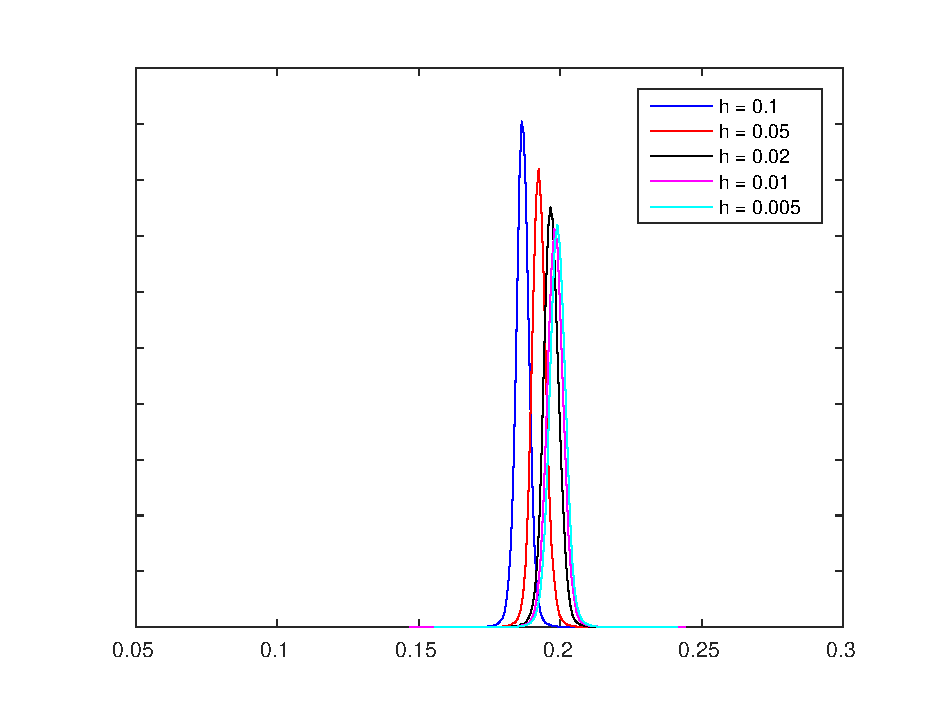
\includegraphics[width=1\linewidth]{plots/FitzNagNoNoise/TopLeft}
	\end{subfigure}
	\hspace*{.66\textwidth}\quad
	
	\begin{subfigure}{0.32\linewidth}
		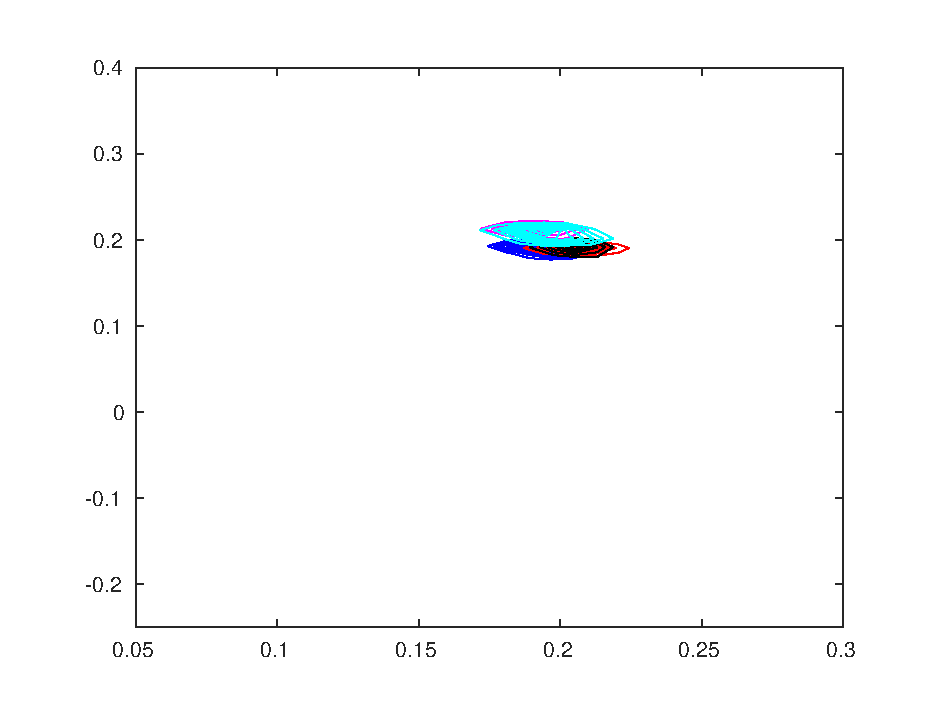
\includegraphics[width=1\linewidth]{plots/FitzNagNoNoise/MiddleLeft}
	\end{subfigure}
	\begin{subfigure}{0.32\linewidth}
		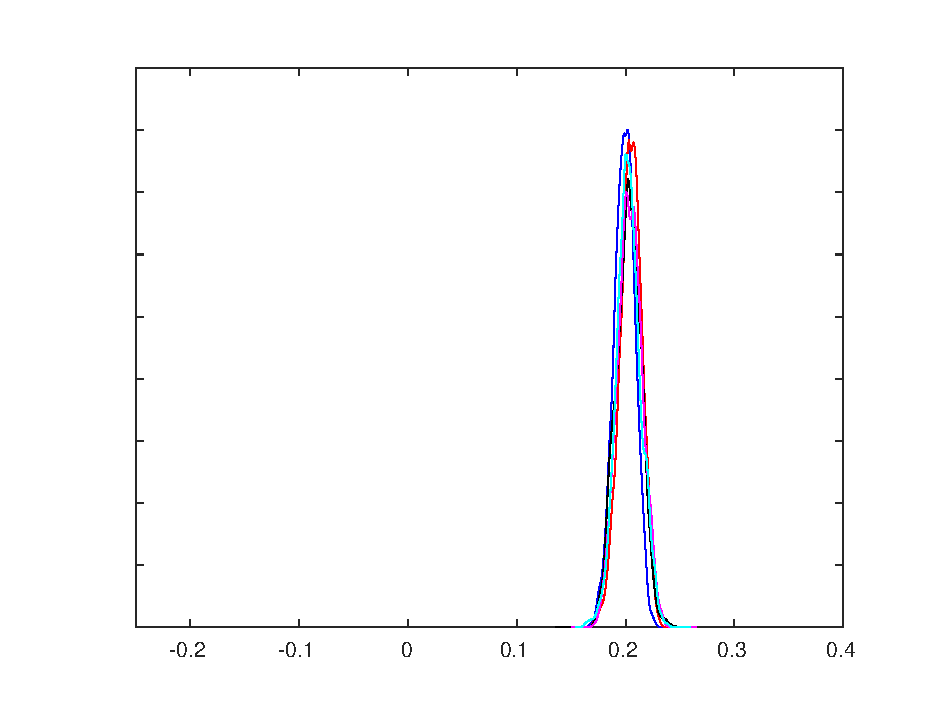
\includegraphics[width=1\linewidth]{plots/FitzNagNoNoise/MiddleMiddle}
	\end{subfigure}
	\hspace*{.33\textwidth}\quad
	
	\begin{subfigure}{0.32\linewidth}
		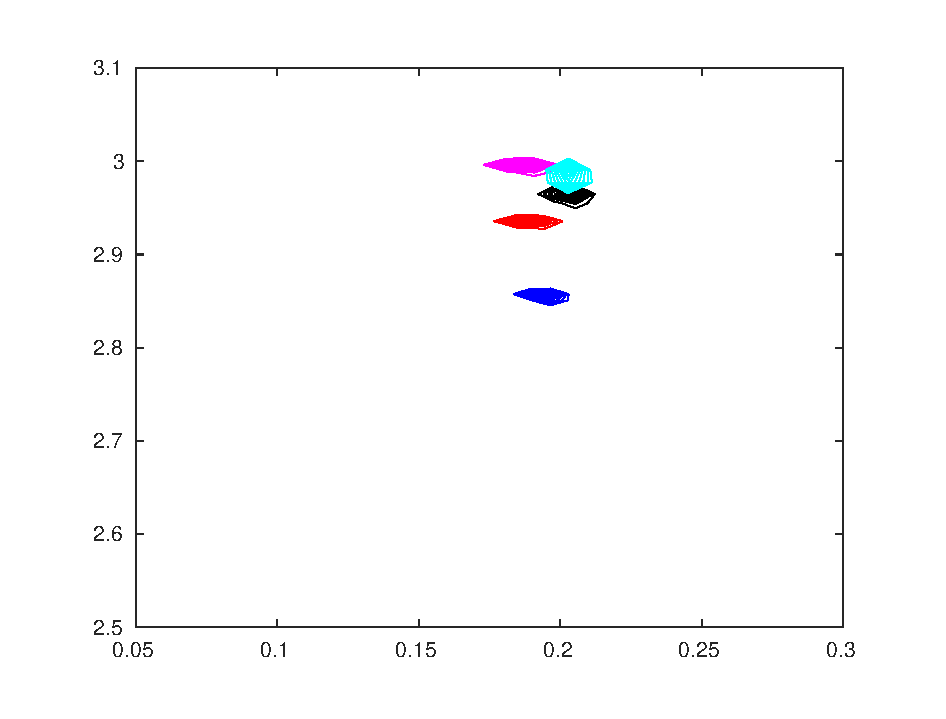
\includegraphics[width=1\linewidth]{plots/FitzNagNoNoise/BottomLeft}
	\end{subfigure}
	\begin{subfigure}{0.32\linewidth}
		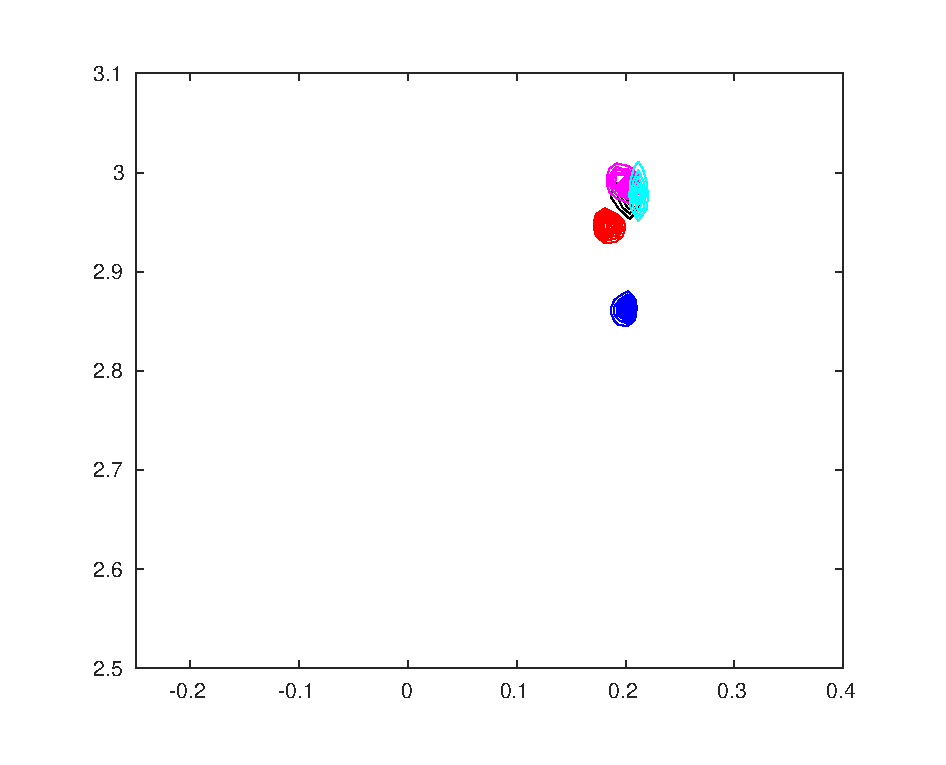
\includegraphics[width=1\linewidth]{plots/FitzNagNoNoise/BottomMiddle}
	\end{subfigure}
	\begin{subfigure}{0.32\linewidth}
		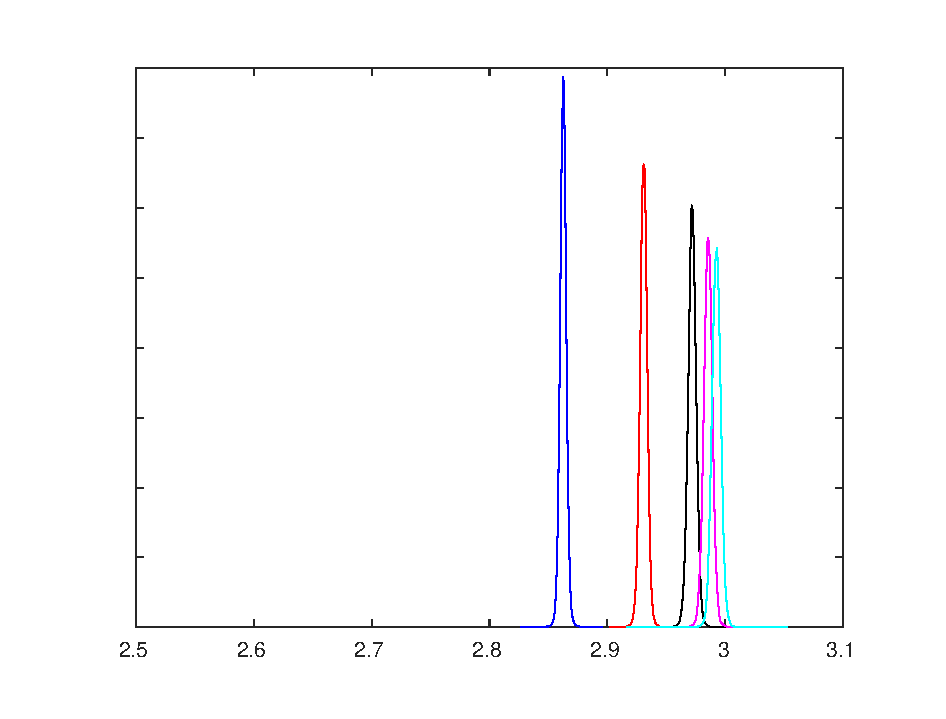
\includegraphics[width=1\linewidth]{plots/FitzNagNoNoise/BottomRight}
	\end{subfigure}
	\caption{Marginal distributions for $\theta$ obtained with the deterministic solver. The posterior distributions are clearly concentrated and mutually singular.}
	\label{fig:FitzNagDet}
\end{figure}

\begin{figure}[t]
	\centering
	\begin{subfigure}{0.33\linewidth}
		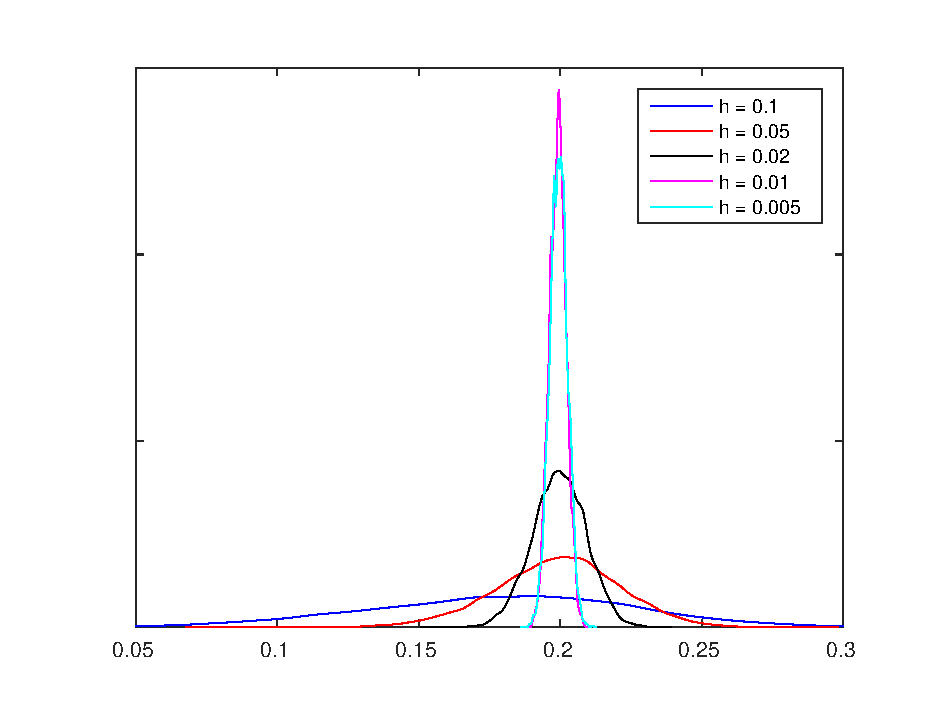
\includegraphics[width=1\linewidth]{plots/FitzNagNoise/TopLeft}
	\end{subfigure}
	\hspace*{.66\textwidth}\quad
	
	\begin{subfigure}{0.32\linewidth}
		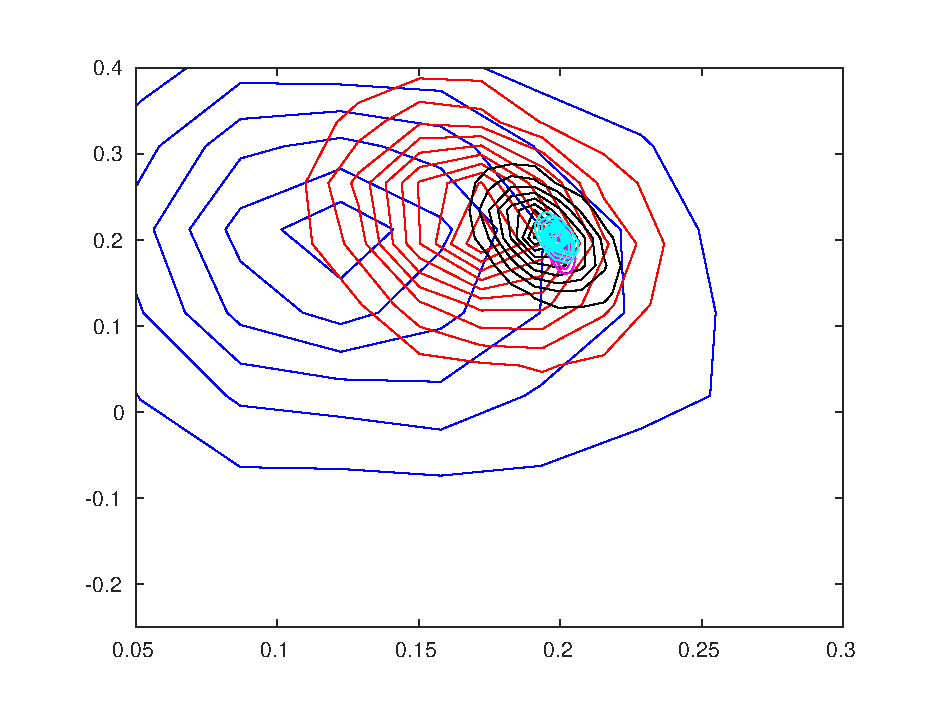
\includegraphics[width=1\linewidth]{plots/FitzNagNoise/MiddleLeft}
	\end{subfigure}
	\begin{subfigure}{0.32\linewidth}
		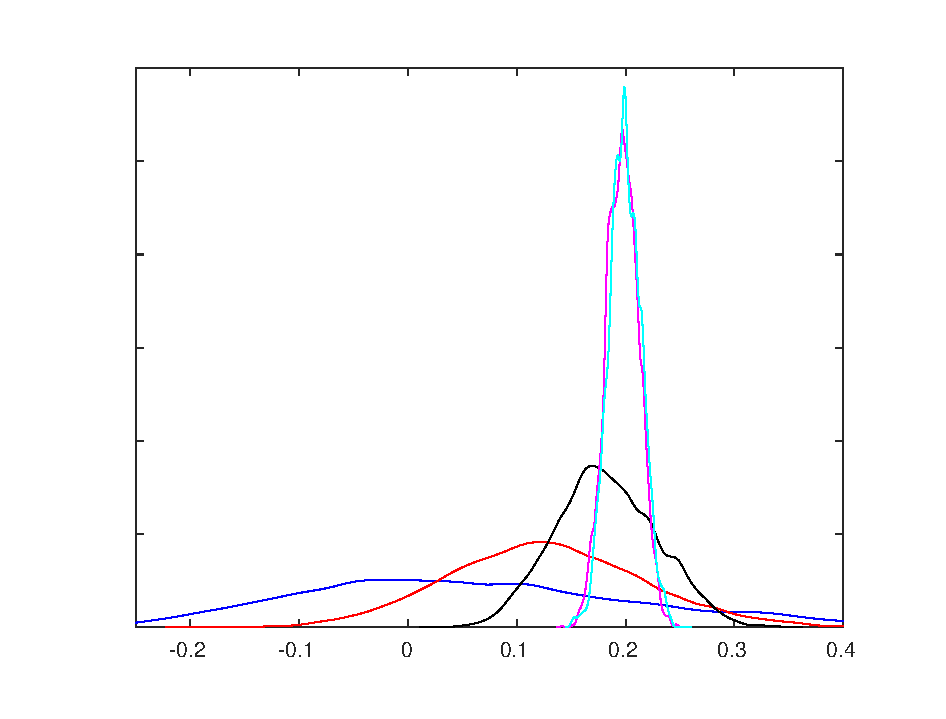
\includegraphics[width=1\linewidth]{plots/FitzNagNoise/MiddleMiddle}
	\end{subfigure}
	\hspace*{.33\textwidth}\quad
	
	\begin{subfigure}{0.32\linewidth}
		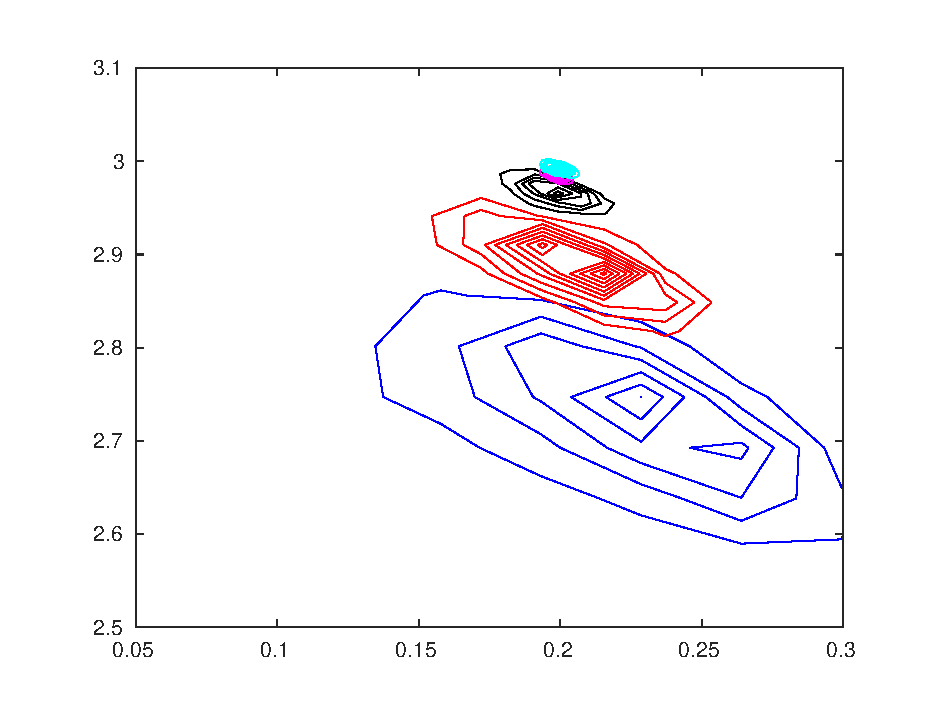
\includegraphics[width=1\linewidth]{plots/FitzNagNoise/BottomLeft}
	\end{subfigure}
	\begin{subfigure}{0.32\linewidth}
		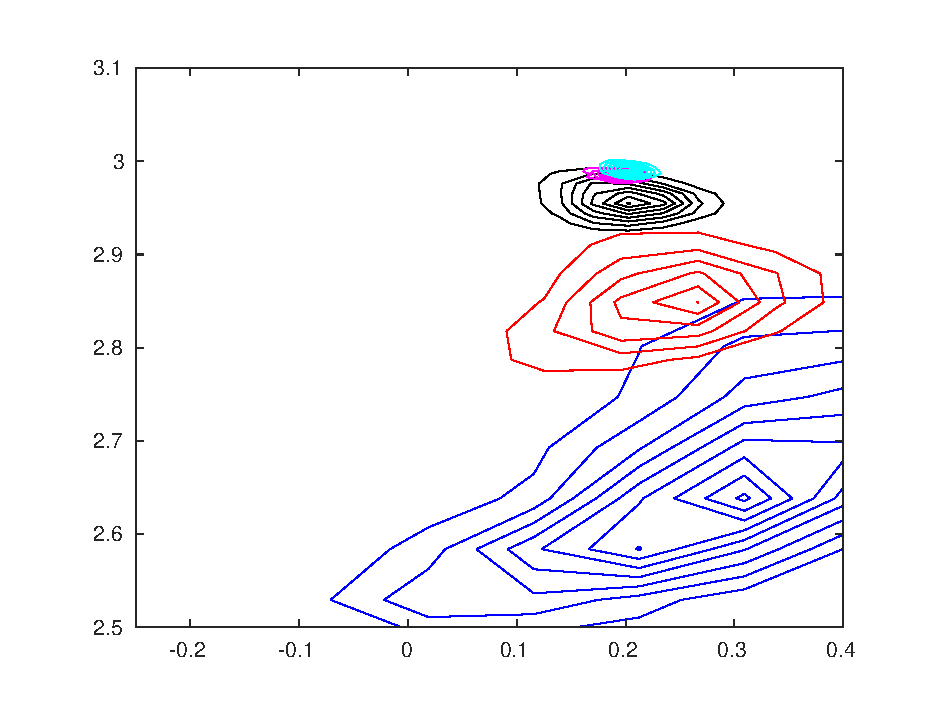
\includegraphics[width=1\linewidth]{plots/FitzNagNoise/BottomMiddle}
	\end{subfigure}
	\begin{subfigure}{0.32\linewidth}
		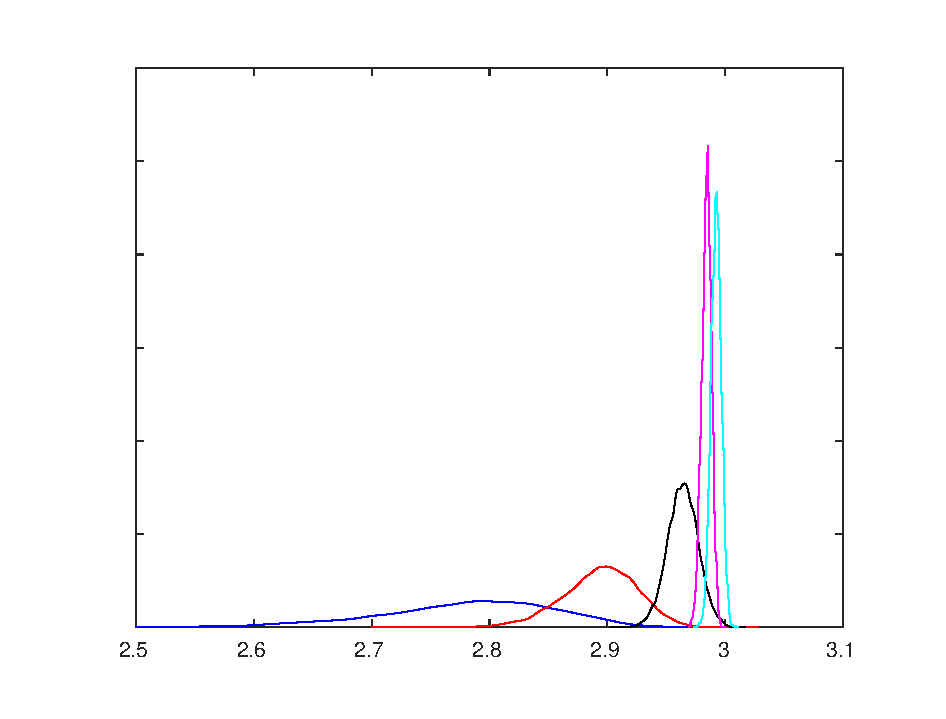
\includegraphics[width=1\linewidth]{plots/FitzNagNoise/BottomRight}
	\end{subfigure}
	\caption{Marginal distributions for $\theta$ obtained with the probabilistic solver. The posterior distributions account for the numerical error.}
	\label{fig:FitzNagProb}
\end{figure}

